\documentclass{article}
\usepackage[utf8]{inputenc}
\usepackage[a4paper,margin=1in]{geometry}
\usepackage{graphicx}
\usepackage{hyperref}
\usepackage{float}

\hypersetup{
    colorlinks=true,
    linkcolor=blue,
    filecolor=blue,      
    urlcolor=red,
}

\title{In-Class Kaggle Competition Instructions}
\author{Zachary Blanks}

\begin{document}
\maketitle

\section{Overview}\label{overview}

In this write-up I'm going to show you how you can get a working Kaggle
competition that could be hosted in a classroom setting. For more
information on how the file system works in this repository, take a look
at the \href{README.md}{README}. This guide breaks a few major
components: getting the data (optional; already provided in
\href{/data}{data} folder if you don't want to run the code) and setting
the necessary parts of a Kaggle competition.

\section{Getting the Data (optional)}\label{getting-the-data-optional}

For this Kaggle competition we're going to be using the Iris data set
that is provided natively in the Scikit-learn package. If you want to
see what the data looks like, run the code provided in the
\href{kaggle-competition-data-benchmark.ipynb}{notebook} up to the
``Running the Benchmark'' section of the notebook.

\section{Starting the Kaggle
Competition}\label{starting-the-kaggle-competition}

To run your own in-class competition there are a number of steps that
have to be taken. None of them are difficult, but you have to go through
them for Kaggle to consider it a ``valid'' competition.

\subsection{Defining the First
Competition}\label{defining-the-first-competition}

The first thing that you will have to do is go to Kaggle's home
``competition'' website. This can be found at
\href{https://www.kaggle.com/competitions}{competitions}. To start your
own competition you will need to either sign into an existing Kaggle
account or make your own. I will proceed with this guide under the
assumption that you do not have a Kaggle account.

\subsubsection{Making a Kaggle Account}\label{making-a-kaggle-account}

To make a Kaggle account, click the ``Sign In'' link at the top right of the image

\begin{figure}[H]
    \centering
    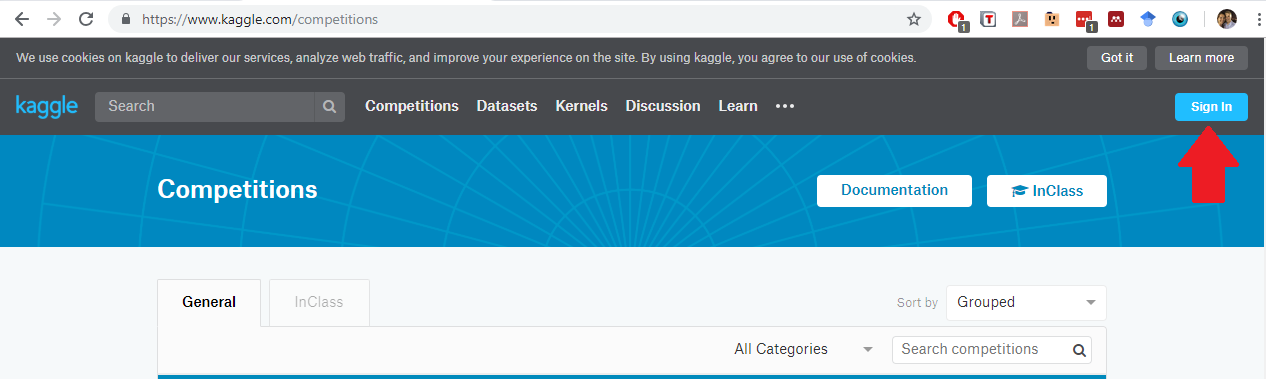
\includegraphics[width=\linewidth]{figures/sign-in.PNG}
\end{figure}

After clicking the link you should see

\begin{figure}[H]
    \centering
    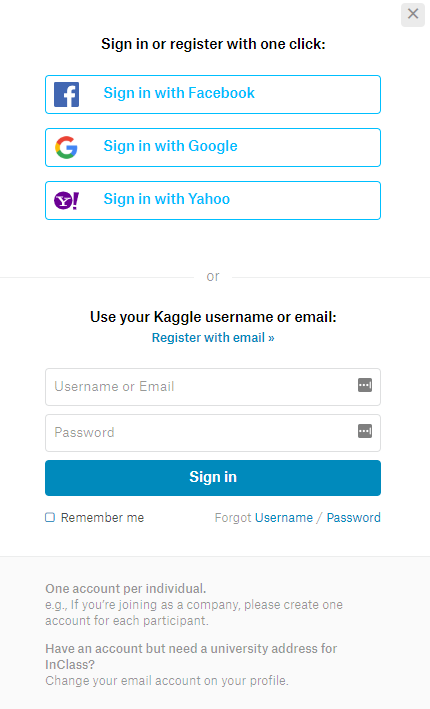
\includegraphics[width=\linewidth]{figures/sign-in-click.PNG}
\end{figure}

You can select any way that you would like to register an account with
Kaggle. Follow the instructions that Kaggle provides.

After you have signed into your account, click the link ``InClass''
link: 

\begin{figure}[H]
    \centering
    
\includegraphics[width=\linewidth]{figures/in-class-link.PNG}
\end{figure}

This will take you a new page with the URL:
\url{https://www.kaggle.com/about/inclass/overview}. To create the
competition, click the button, ``Create new competition'' as shown in
the picture

\begin{figure}[H]
    \centering
    
\includegraphics[width=\linewidth]{figures/create-competition-page.PNG}
\end{figure}

After clicking this link, it should take you to the link
\url{https://www.kaggle.com/competitions/new}. On this page we will need
to do a few things:

\begin{enumerate}
    \item Enter a title at the point where it asks us to type this
    \item Provide a brief description of the competition
    \item Create a competition URL
\end{enumerate}

The descriptive title will be ``Example Kaggle Competition.'' The brief
description will be: ``Example Kaggle competition'', and the competition
URL will be ``example-competition.'' \textbf{Make sure you click those
blocks.} I made that mistake when I made my first competition and I kept
getting an error I didn't understand. After you have provide all of
those links click the ``Create Competition'' button. The locations to
click are shown in the figure below

\begin{figure}[H]
    \centering
    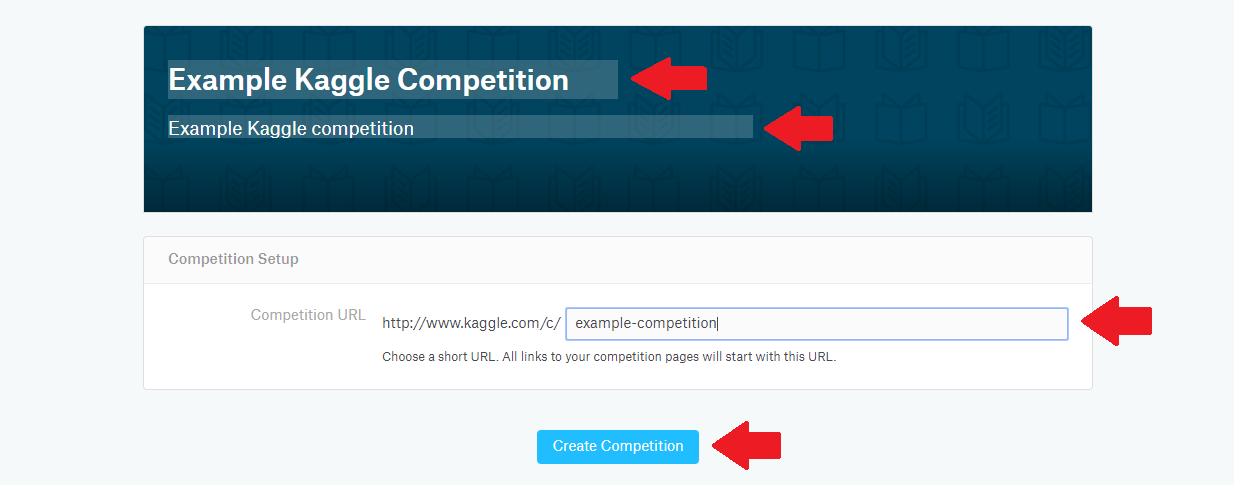
\includegraphics[width=\linewidth]{figures/start-competition.PNG}
\end{figure}

Once you have done all of those steps, you should now be at a page with
a URL \url{https://www.kaggle.com/c/example-competition}. It can be a
bit overwhelming all the things that have to be done to make the
competition work, but we're going to break it into bite-sized pieces so
that we understand everything we need to do.

First, click on the ``Host'' tab and in the ``Host'' tab, click ``Launch
Checklist.'' It should look like

\begin{figure}[H]
    \centering
    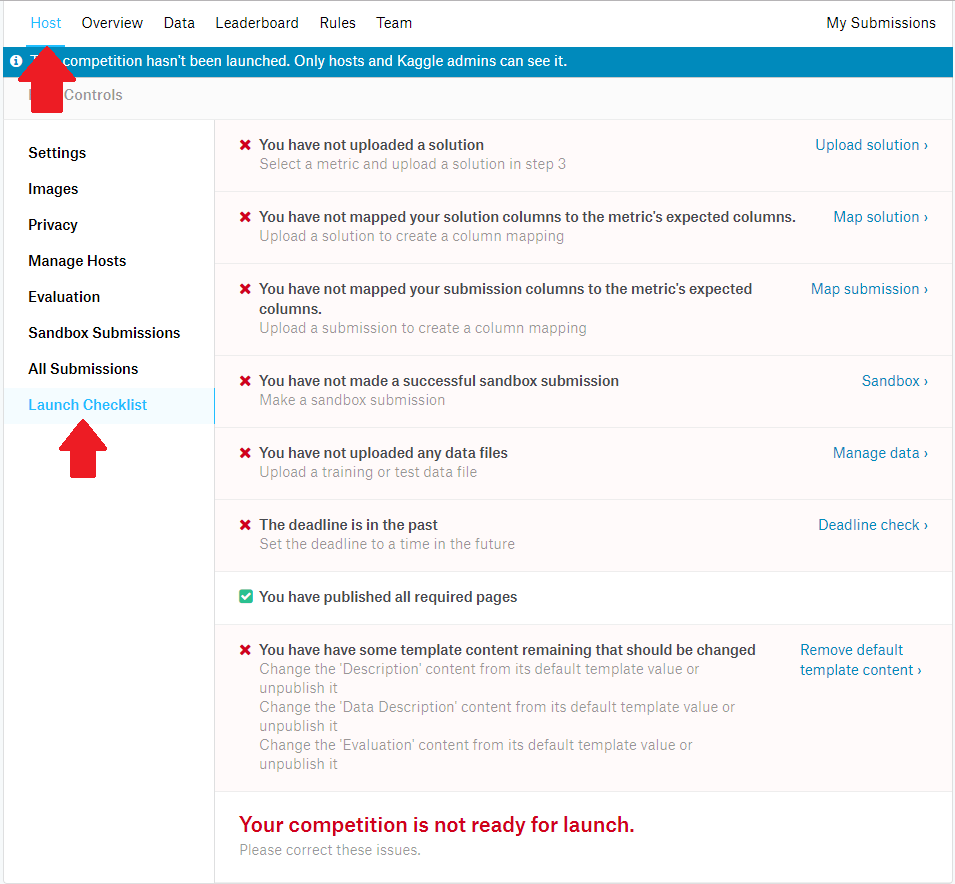
\includegraphics[width=\linewidth]{figures/launch-checklist.PNG}
\end{figure}

The best approach to get this competition running is to just follow each
step of the checklist. Therefore, the firs thing we're going to do is
upload a solution.

\subsection{Uploading the Solution}\label{uploading-the-solution}

To upload the solution click ``Upload solution link in the checklist''

\begin{figure}[H]
    \centering
    
\includegraphics[width=\linewidth]{figures/upload-solution-link.PNG}
\end{figure}

After clicking that link, you will be taken to the URL
\url{https://www.kaggle.com/c/example-competition/host\#evaluation}. For
this component of the competition, we need to select a scoring metric,
we need to provide the solution file, and we need to give an example of
a valid submission. For the scoring metric, select
``CategorizationAccuracy.'' This can be found my clicking the drop-down
in the ``Scoring Metric'' box. Aftering taking this action, your page
should look like this

\begin{figure}
    \centering
    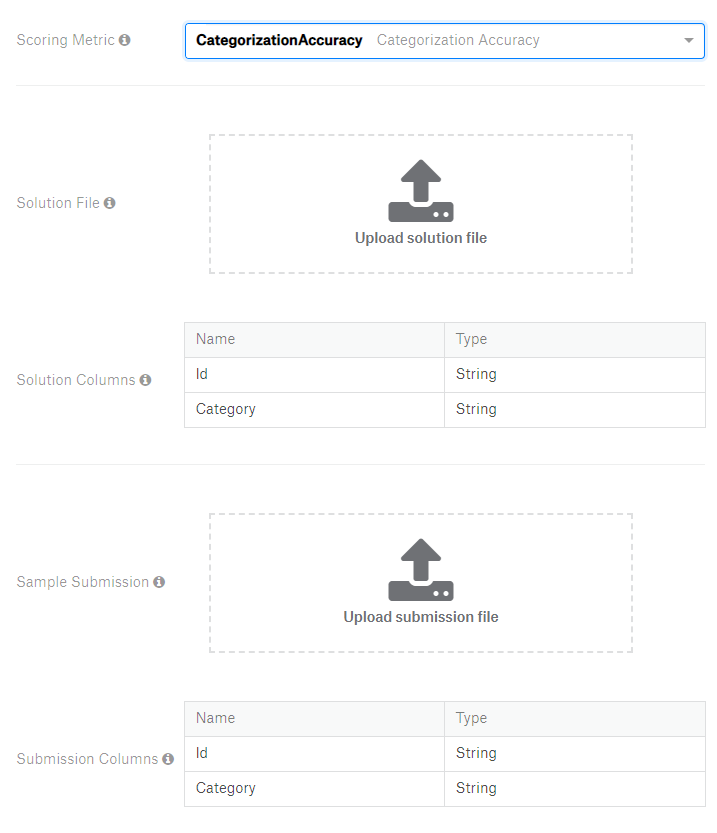
\includegraphics[width=\linewidth]{figures/category-acc.PNG}
\end{figure}

Next we need to upload the solution file. This can be found in the file
\texttt{data/solution\_file.csv} in the \href{/data}{data} folder which
is provided with the repository. To upload the file click ``Upload
solution file'' and provide a link to the solution file. If this was
done correctly, you should see

\begin{figure}[H]
    \centering
    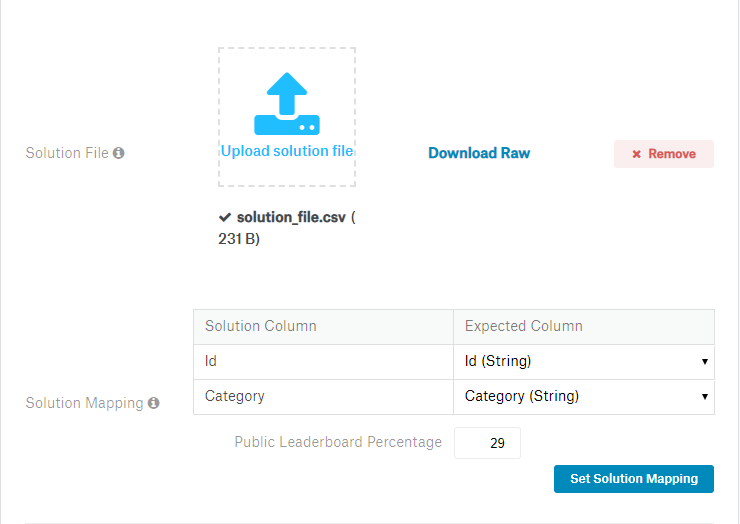
\includegraphics[width=\linewidth]{figures/solution-file-result.PNG}
\end{figure}

Once the solution file has been loaded, you need to click ``Set Solution
Mapping.'' Basically what this does is map the submission to the
expected column format. Once this has been you should see

\begin{figure}[H]
    \centering
    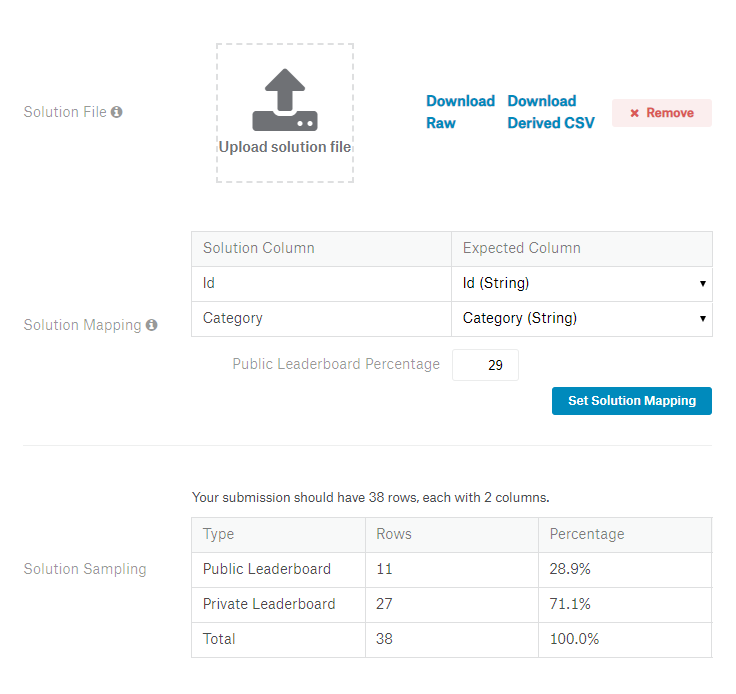
\includegraphics[width=\linewidth]{figures/solution-mapping.PNG}
\end{figure}

Finally, we need to provide a valid sample submission. This has been
provided with the file \texttt{data/valid\_submission.csv}. Again click
the ``Upload submission file'' to provide the valid submission. We also
need to click the ``Set Submission Mapping''. This time though we need
to provide information for the ``Validator''. What is Kaggle is doing is
validating the data that has been provided in the submission and ensures
that it can be mapped to the expected format. For the ``Id'' column
click click: Non-negative Integers \{0, 1, \ldots{}, 100000\} since we
have 38 samples in the test set, and for the ``Category'' select
Integers between 0 and 20 since we have three labels in the data. After
you have set those categories, remember to click the ``Set Submission
Mapping'' button. If this is done correctly it should look like

\begin{figure}[H]
    \centering
    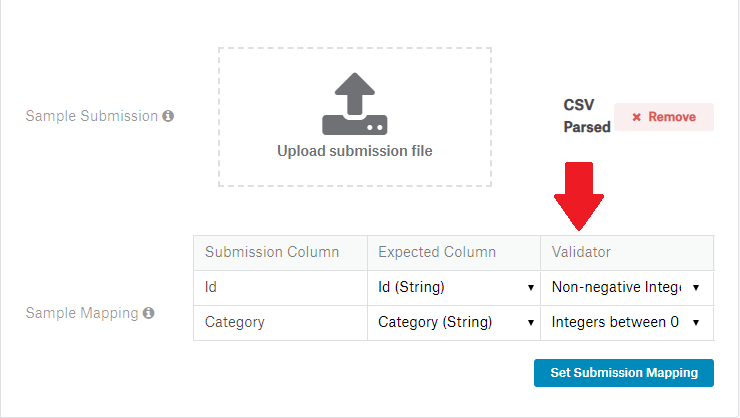
\includegraphics[width=\linewidth]{figures/submission-mapping.PNG}
\end{figure}

To check that everything work correctly for this part of the process
let's return to the ``Launch Checklist.''

If the steps above were followed correctly, after clicking to the
``Launch Checklist'', you should see

\begin{figure}[H]
    \centering
    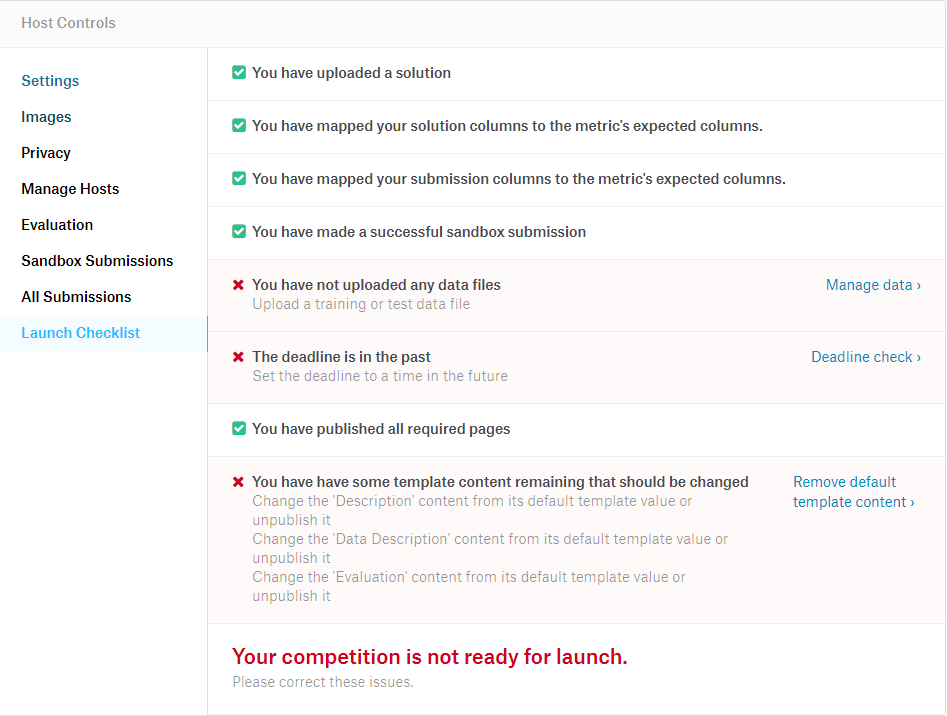
\includegraphics[width=\linewidth]{figures/launch-checklist-post-evaluation.PNG}
\end{figure}

The next step is to upload data files. This can be done by clicking the
``Manage data'' link

\begin{figure}[H]
    \centering
    
\includegraphics[width=\linewidth]{figures/manage-data.PNG}
\end{figure}

\subsection{Manage Data}\label{manage-data}

After clicking the link you should be at the URL
\url{https://www.kaggle.com/c/example-competition/data}. To upload the
first version of the data files, click the button ``Upload first
version''

\begin{figure}[H]
    \centering
    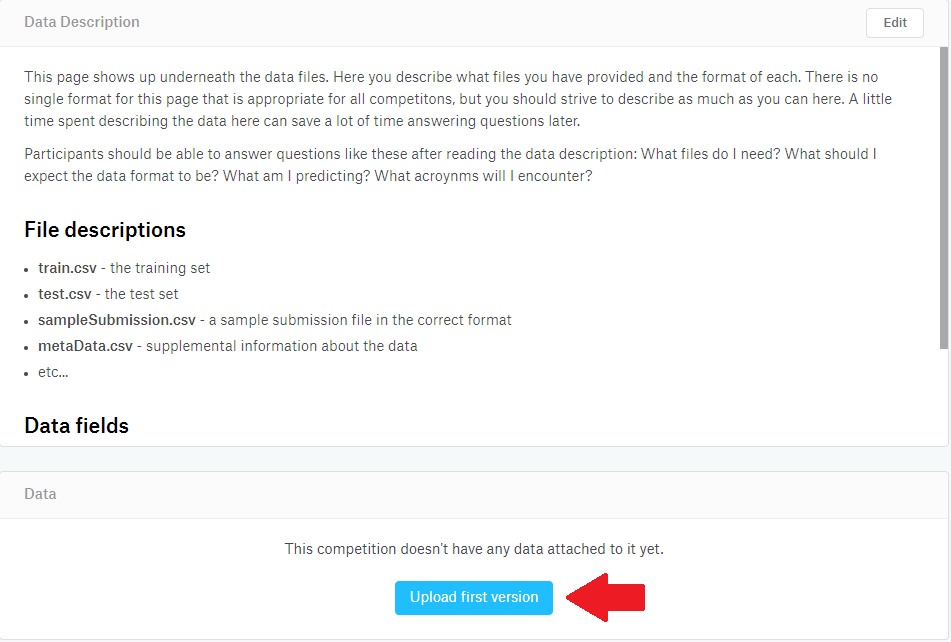
\includegraphics[width=\linewidth]{figures/upload-data.PNG}
\end{figure}

For this part, we're going to upload the following files:

\begin{enumerate}
\item
  \texttt{data/X\_train.csv}
\item
  \texttt{data/X\_test.csv}
\item
  \texttt{data/y\_train.csv}
\item
  \texttt{data/submission\_file.csv}
\end{enumerate}

You should not load the test labels because that defeats the point of
the competition. The reason that we're uploading the
\texttt{submission\_file.csv} is because we want the user to understand
what a valid submission looks like. To upload these files select them
from the \href{/data}{data} folder and click the link ``Select Files to
Upload.'' After doing so, you will have to provide ``Version notes.''
For this instance, just type: ``First version.'' After taking these
steps it should look like

\begin{figure}[H]
    \centering
    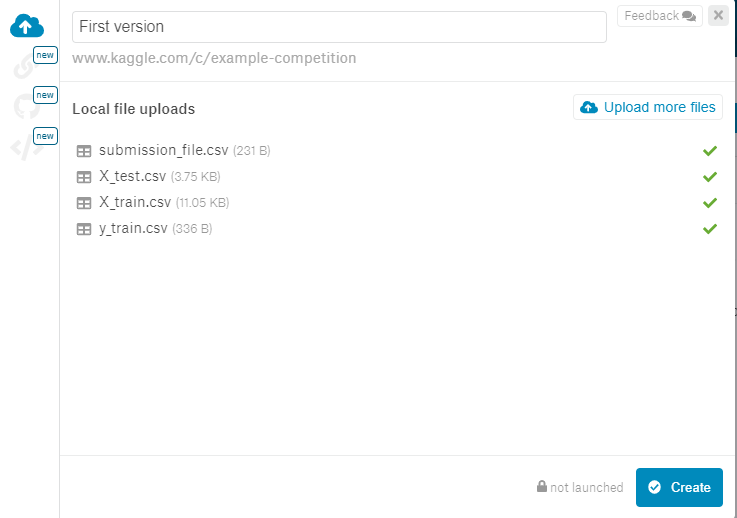
\includegraphics[width=\linewidth]{figures/data-upload-result.PNG}
\end{figure}

One quick note, Kaggle, as I discovered expects the uploaded .csv files
to have headers otherwise it will treat the first row of data as the
header. There might be a way to adjust this setting, but it's probably
easier to just provide a header.

Let's again return to the Launch Checklist to see what's left to getting
this competition up and running.

After uploading the data file, the Launch Checklist should now look like

\begin{figure}[H]
    \centering
    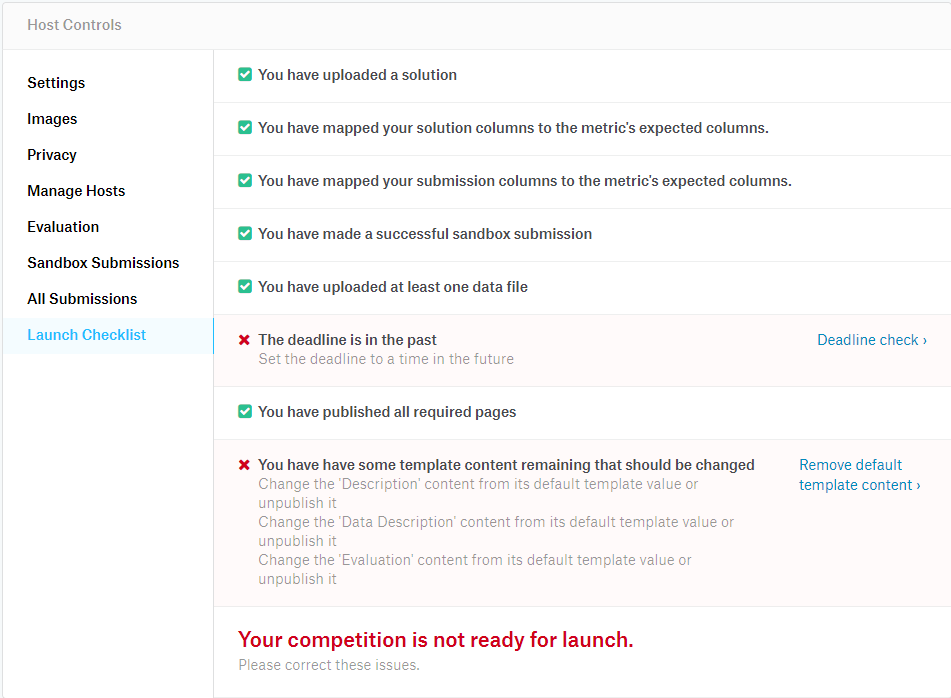
\includegraphics[width=\linewidth]{figures/launch-checklist3.PNG}
\end{figure}

The next thing we need to do is update the competition deadline.

\subsection{Competition Deadline}\label{competition-deadline}

To update the competition deadline, click the ``Deadline check'' link.
After clicking the link you should see the URL:
\url{https://www.kaggle.com/c/example-competition/host}. There are many
things that could be changed on this page, but the primary thing we have
to change is the ``Deadline.'' Since this guide was written on
2019-02-24, I am going to set the deadline to 2019-03-02. When doing a
competition in a real situation though you should take of course account
for how long you want it to go. After adjust the date you should see

\begin{figure}[H]
    \centering
    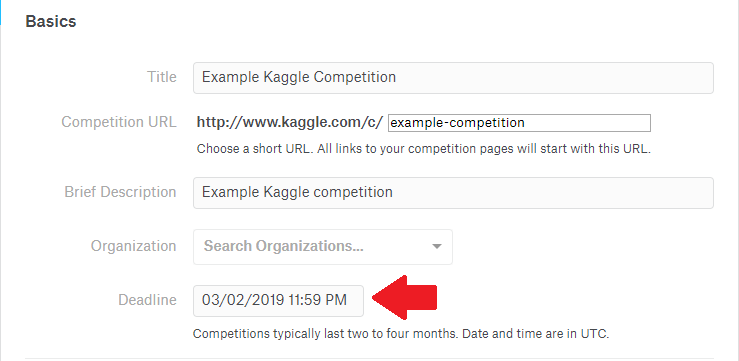
\includegraphics[width=\linewidth]{figures/date-adjustment.PNG}
\end{figure}

Make sure to click ``Save changes,'' and let's go back to the Launch
Checklist.

After adjusting the date, you should now see

\begin{figure}[H]
    \centering
    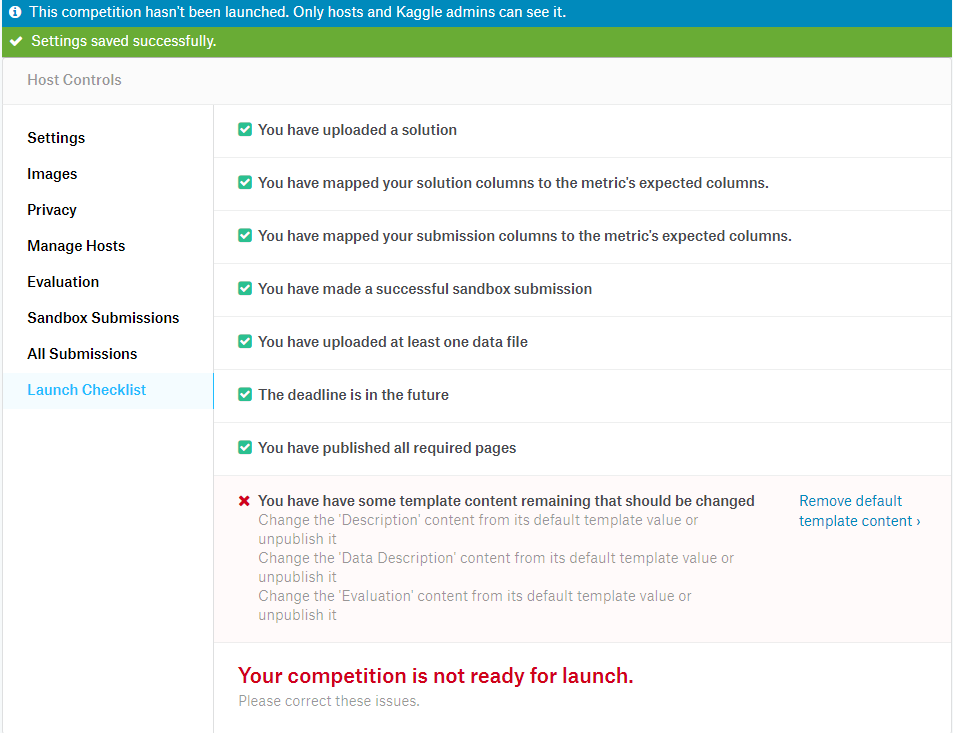
\includegraphics[width=\linewidth]{figures/launch-checklist4.PNG}
\end{figure}

All that is left to do is provide information in ``Description'', ``Data
Description'', and ``Evaluation'' tabs. The purpose of these tabs is to
give the users an idea of what the competition entails (i.e.,
motivation, interesting problems they might see, etc.), the format of the
data and what things they should use for the competition, and how their
submissions will be evaluated, respectively. These items are very
dependent upon the particular competition, so I won't provide do
anything on this front. It's something that has to be done for each
competition. However, to ensure that we can have a valid competition,
we're just going to remove the templates. just click ``Remove default
template content.''

\begin{figure}[H]
    \centering
    
\includegraphics[width=\linewidth]{figures/remove-templates.PNG}
\end{figure}

\subsubsection{Description}\label{description}

After clicking the link you should be at the URL
\url{https://www.kaggle.com/c/example-competition/overview}. In the top
right, click ``Edit,'' remove all the writing in the box, and type
``Example description.'' Once this is done, click ``Save''. It should
look like

\begin{figure}[H]
    \centering
    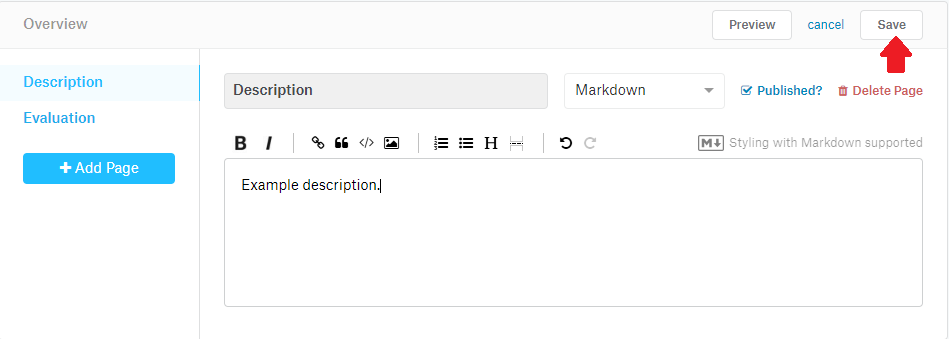
\includegraphics[width=\linewidth]{figures/example-description.PNG}
\end{figure}

\subsubsection{Evaluation}\label{evaluation}

Next we need to adjust the evaluation template. Click on the
``Evaluation'' link in the left tab, and again click ``Edit'' in the top
right. Once again we're going to delete all the writing and just write:
``Example evaluation.'' After this is done, click ``Save.'' It should
look like

\begin{figure}[H]
    \centering
    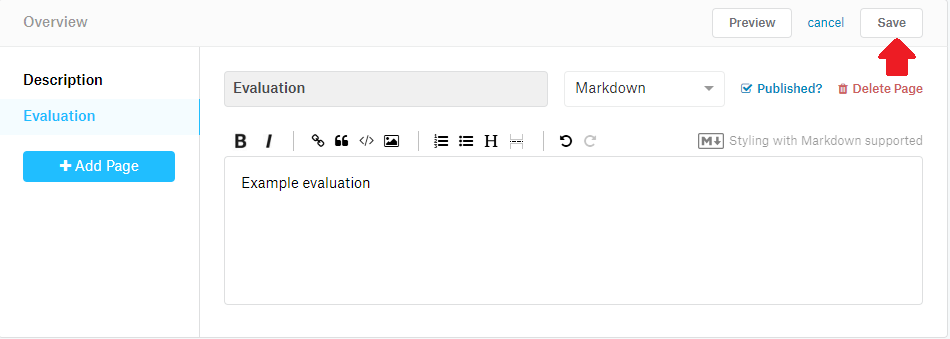
\includegraphics[width=\linewidth]{figures/example-evaluation.PNG}
\end{figure}

\subsubsection{Data Description}\label{data-description}

Finally we need to provide a data description. To do this, click the
``Data'' tab near the top

\begin{figure}[H]
    \centering
    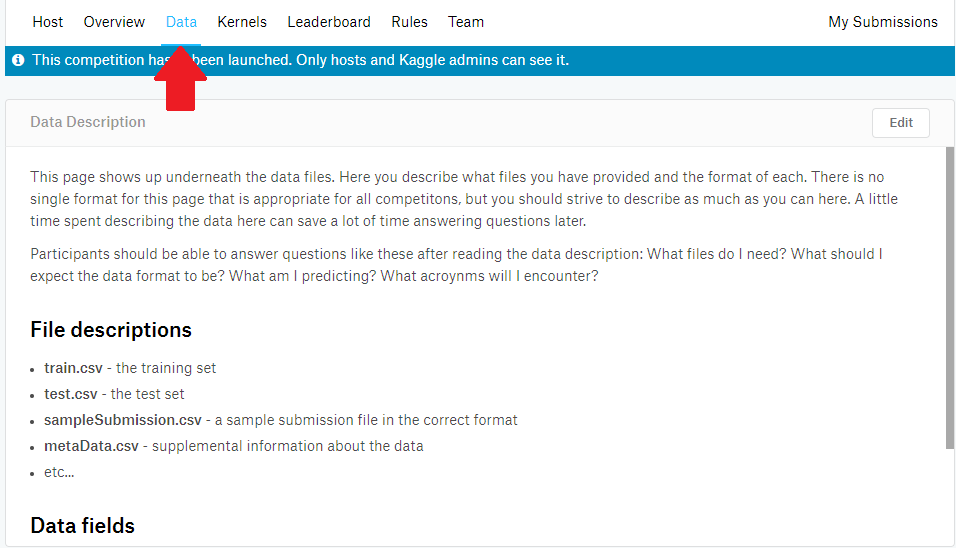
\includegraphics[width=\linewidth]{figures/data-description-link.PNG}
\end{figure}

Again we need to edit the template following the same process. Click
``Edit'', remove the existing text, write ``Example data description'',
and then save.

After taking those three actions, return back to the Launch Checklist by
clicking Host and then Launch Checklist. If all the actions have been
followed, the checklist should now look like

\begin{figure}[H]
    \centering
    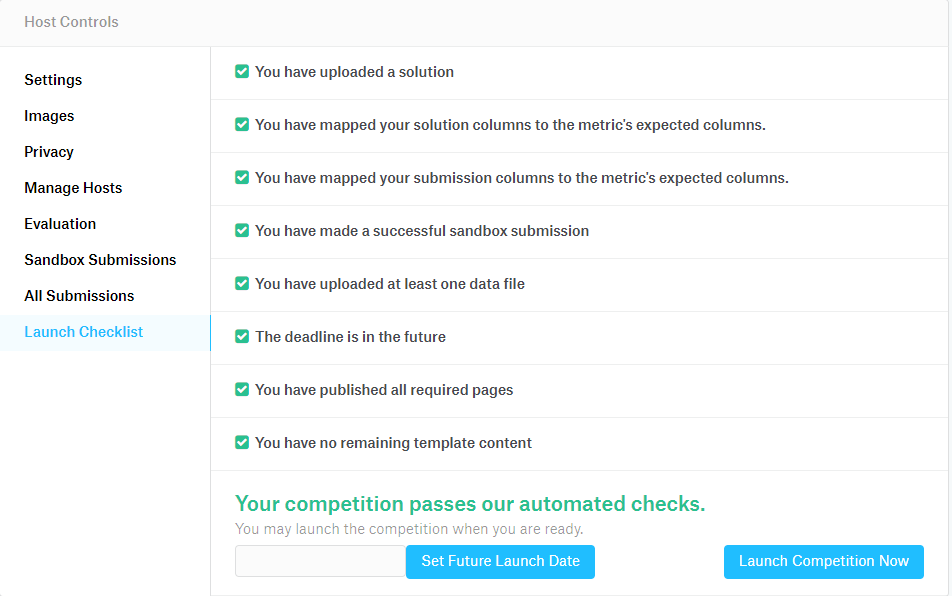
\includegraphics[width=\linewidth]{figures/launch-checklist5.PNG}
\end{figure}

\section{Conclusion}\label{conclusion}

\textbf{Congratulations!} You have now successfully taken all the steps
needed to launch your own Kaggle competition. Of course there are a
number other actions that can make the competition even better. These
options include

\begin{enumerate}
\item
  Privacy -- you can set whether the competition is public or private
\item
  Images -- you can add pictures that make the competition page more
  interesting
\item
  Settings -- we only set the date, but you can also play with the
  number of submissions, whether people can team up, and other things.
\end{enumerate}

In general you'll just have to play around with the page to get the full
scope of actions that you can take, but after following these directions
you have successfully set up a working Kaggle competition.
\end{document}